\chapter{Фрагмент кода}

Фрагмент кода на 15 осмысленных / значимых строк кода (не пробелы, не комментарии, не фигурные скобуи и т.п.) представлен в листинге~\ref{lst:lev_recursion}.

\begin{center}
\captionsetup{justification=raggedright,singlelinecheck=off}
\begin{lstlisting}[label=lst:lev_recursion,caption=Фрагмент кода]
 string inputFilePath = Path.Combine(AppDomain.CurrentDomain.BaseDirectory, "inputfile.txt");
 using (var writer = new StreamWriter(inputFilePath, false)) {
     for (int i = 2; i <= pageLimit + 1; i++) {
         string pageUrl = $"{baseUrl}?page={i}";
         var doc = LoadHtmlDocument(pageUrl);
         if (doc == null) {
         logger.LogCollector($"Cant load page {pageUrl}");
         continue; }
         var recipeLinks = ExtractRecipeLinks(doc);
         Console.WriteLine($"{pageUrl} - {recipeLinks.Count}");
         logger.LogCollector($"Page {i} loaded, links amount: {recipeLinks.Count}");
         if (recipeLinks.Count == 0)
            logger.LogCollector($"Page {i} has no links.");
         else {
             foreach (var link in recipeLinks)
                 writer.WriteLine(link);
             logger.LogCollector($"Page {i} loaded, links amount: {recipeLinks.Count}"); }
    }
}
\end{lstlisting}
\end{center}

\chapter{Информационный граф}

Информационный граф по приведенному листингу кода представлен на рисунке~\ref{fig:IG}.

\begin{figure}[h!]
	\centering
	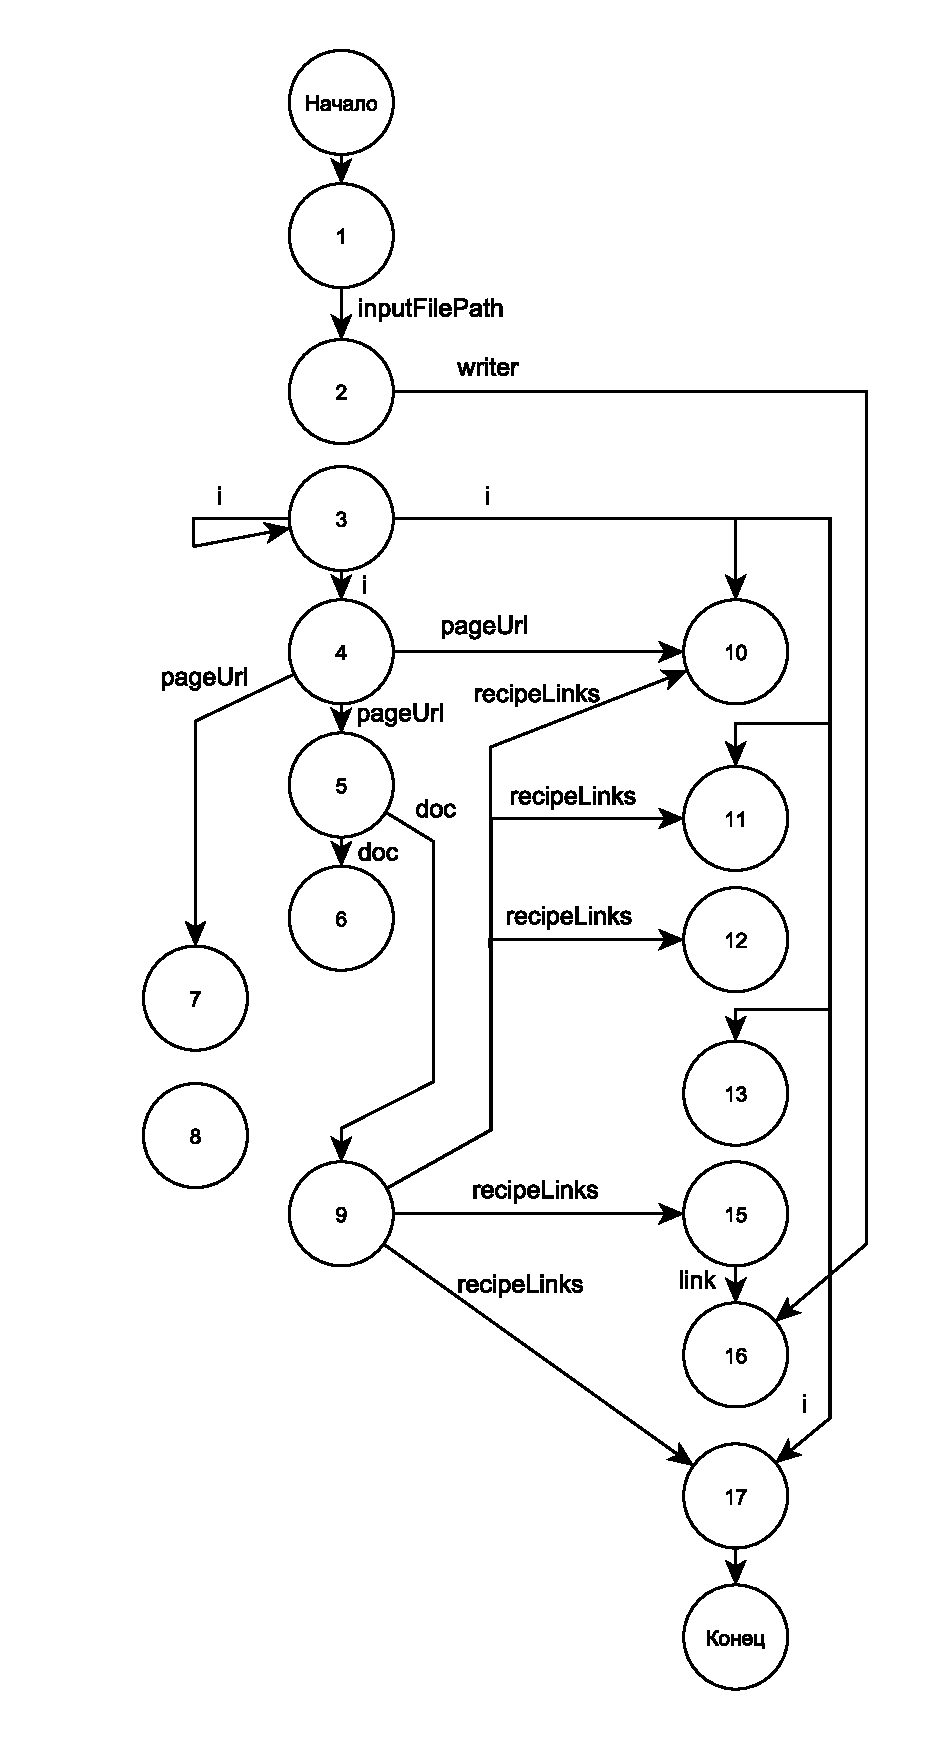
\includegraphics[scale=0.75]{img/InfGraph.eps}
	\caption{Информационный граф}
	\label{fig:IG}
\end{figure}


\chapter{Информационная история}

Информационная история по приведенному листингу кода представлена на рисунке~\ref{fig:II}.

\begin{figure}[h!]
	\centering
	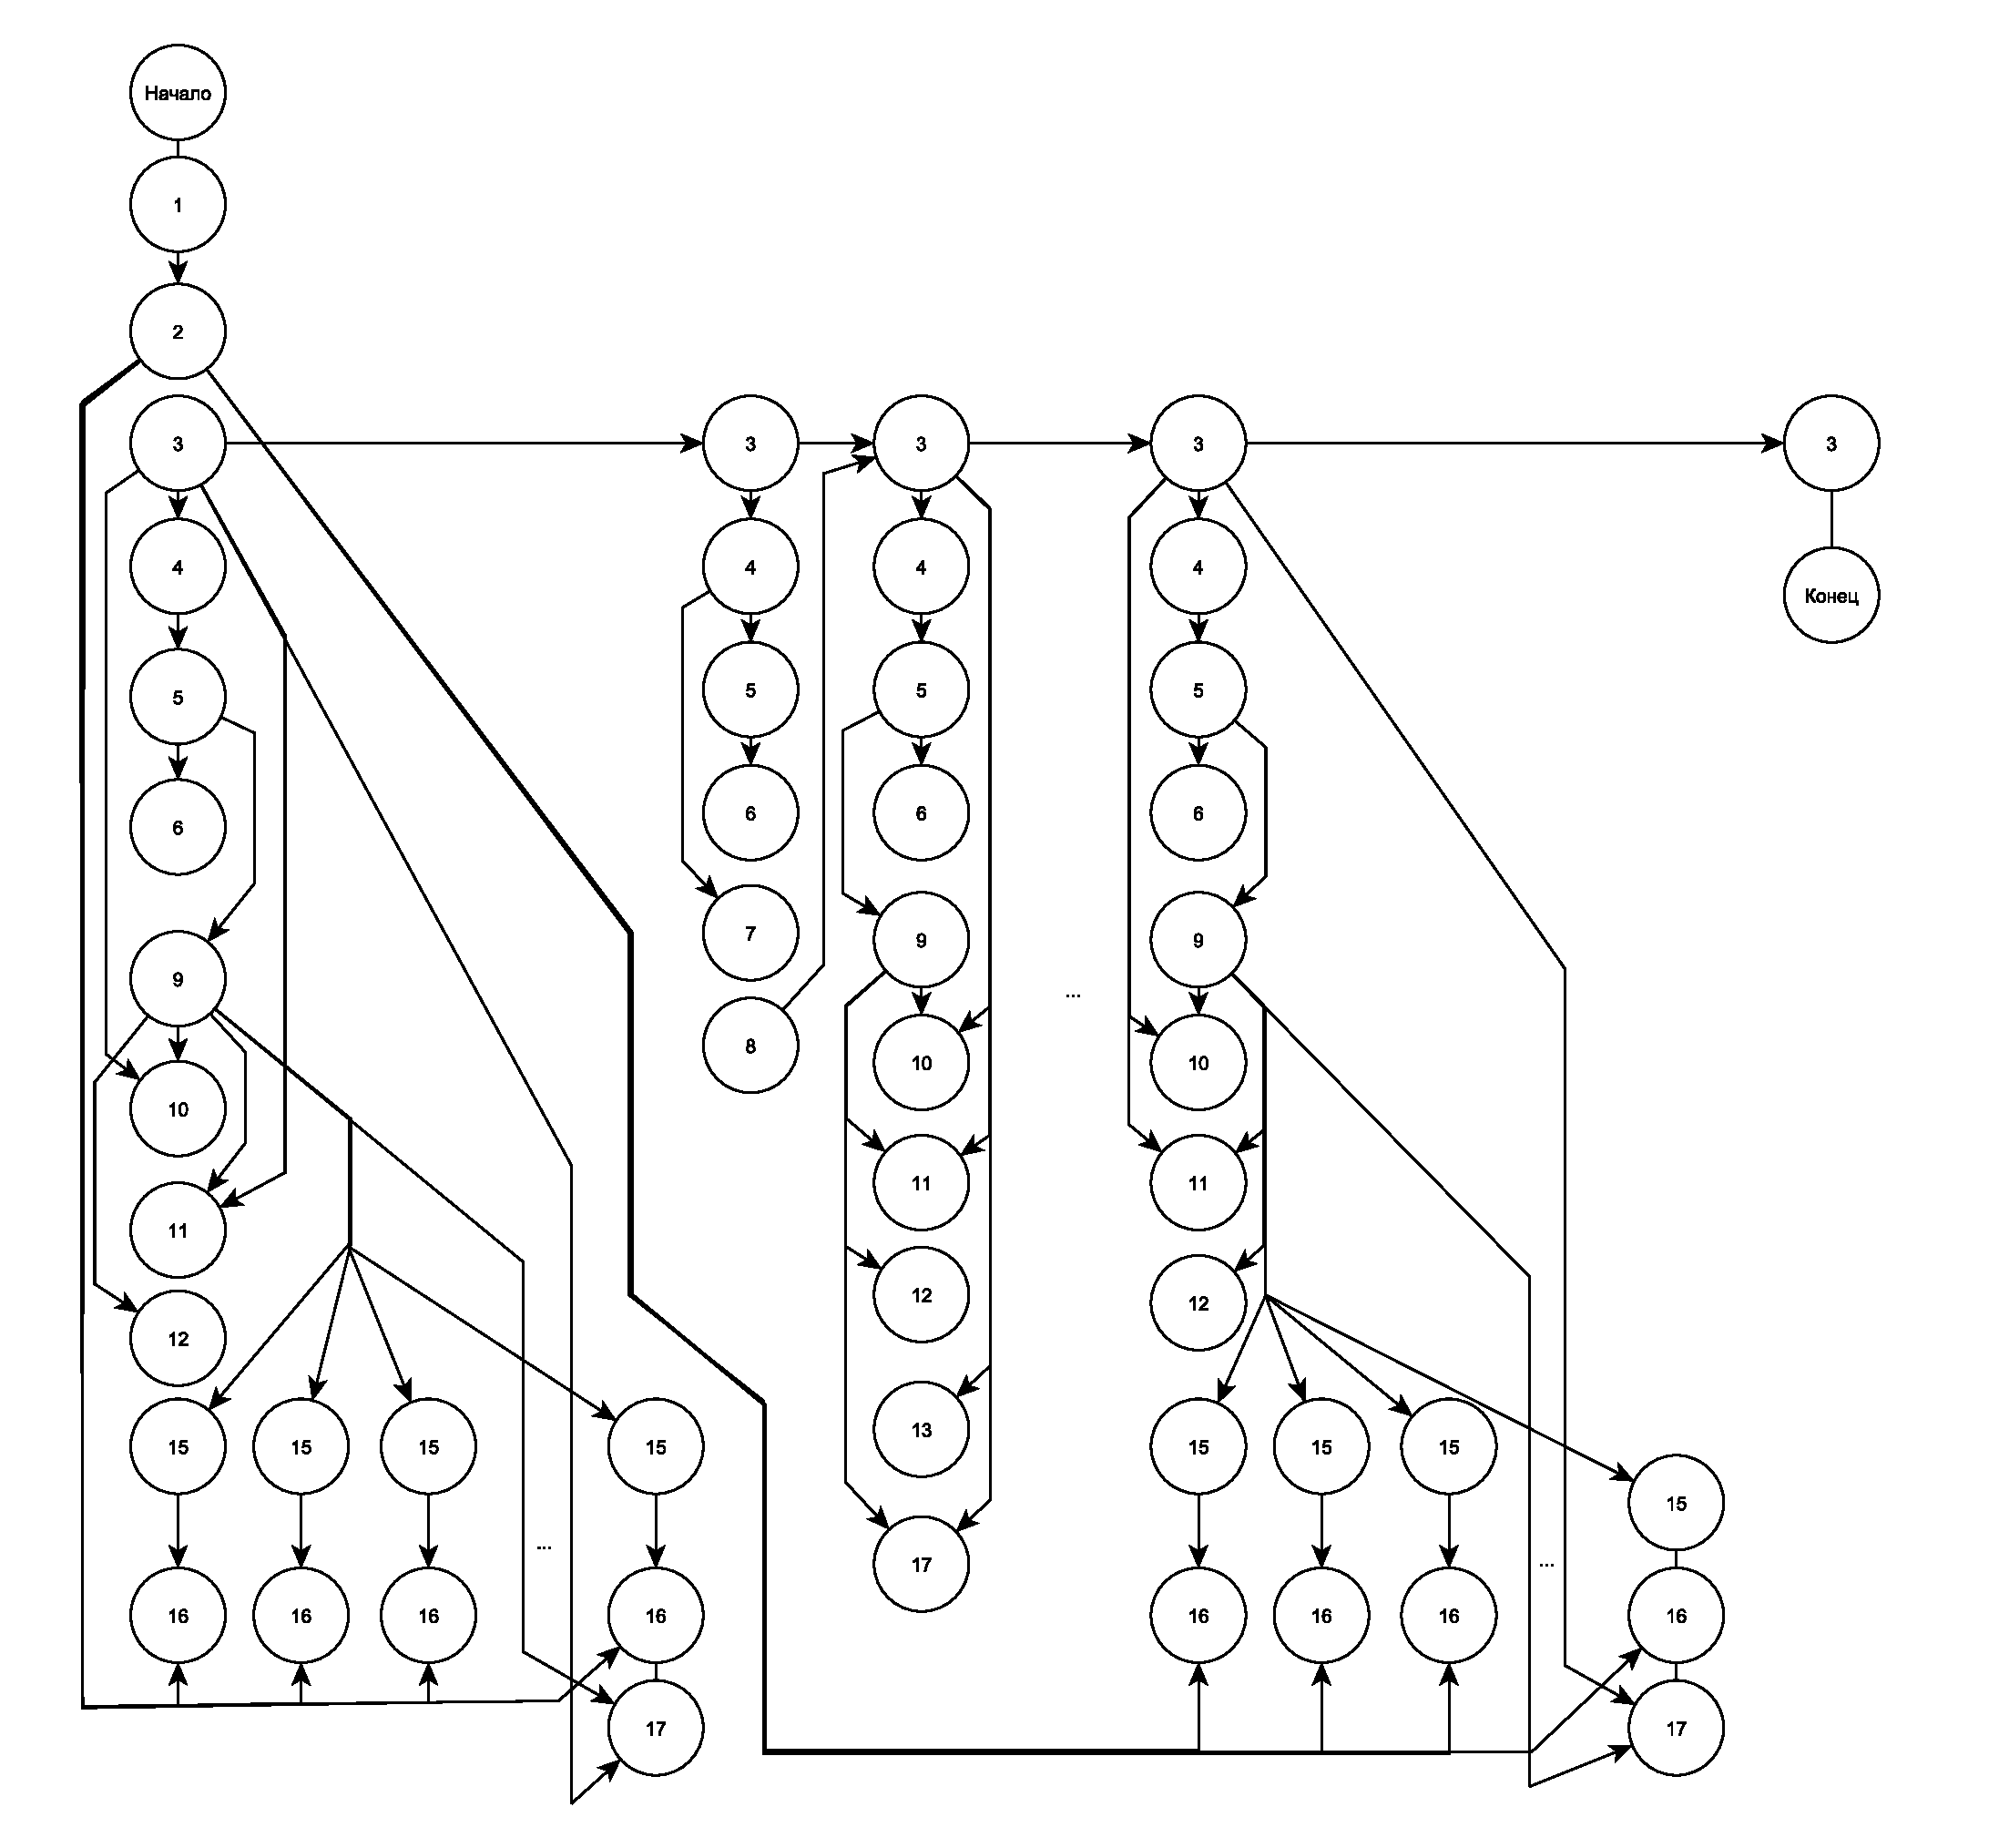
\includegraphics[scale=0.45]{img/InforIstoria.eps}
	\caption{Информационная история}
	\label{fig:II}
\end{figure}

\chapter{Граф управления}

Граф управления по приведенному листингу кода представлен на рисунке~\ref{fig:GY}.

\begin{figure}[h!]
	\centering
	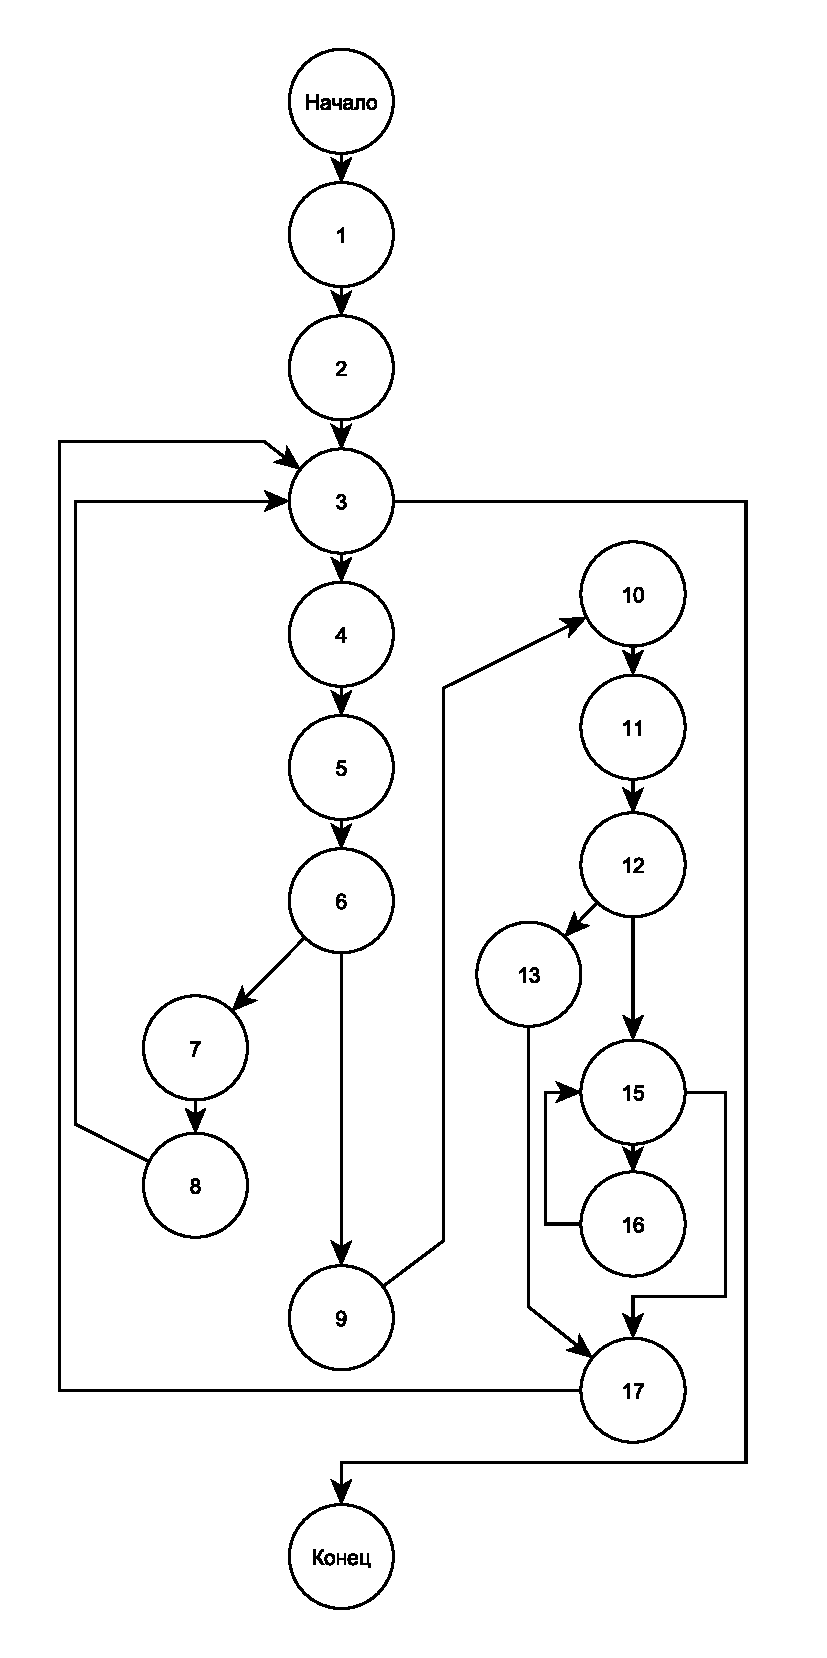
\includegraphics[scale=0.75]{img/GraphYpr.eps}
	\caption{Граф управления}
	\label{fig:GY}
\end{figure}

\chapter{Операционная история}

Операционная история [1] по приведенному листингу кода представлена на рисунке~\ref{fig:OI}.

\begin{figure}[h!]
	\centering
	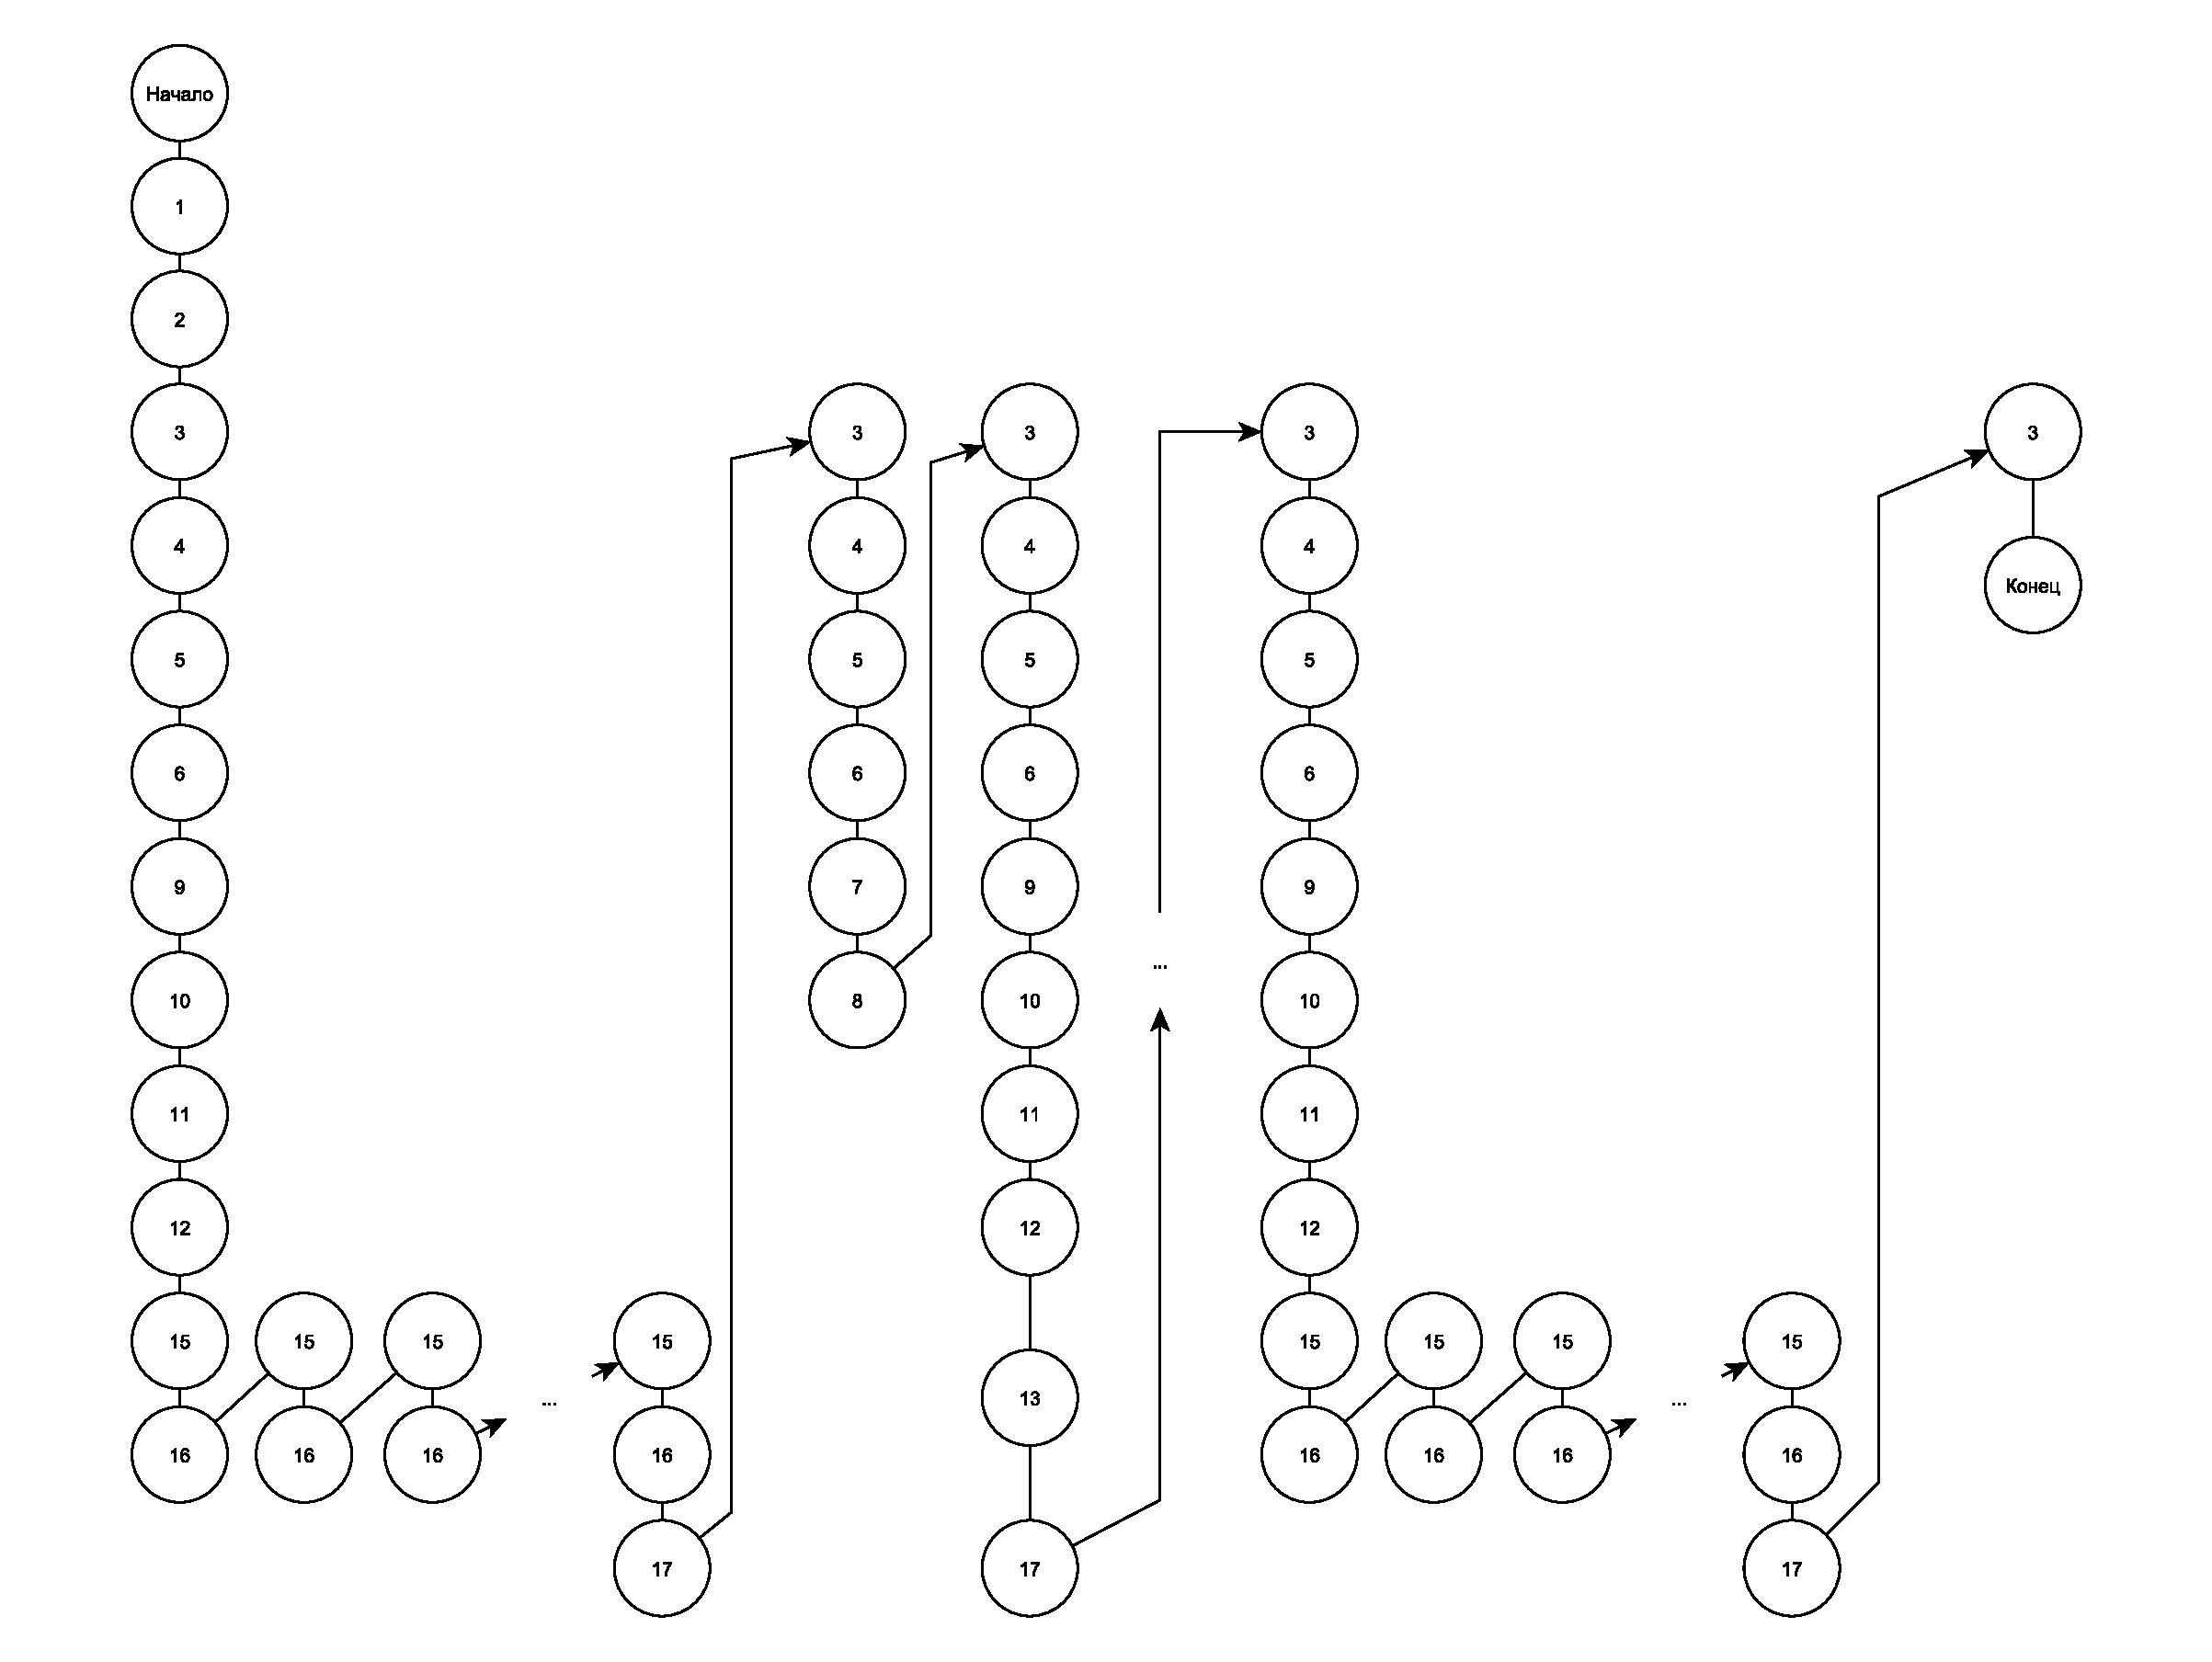
\includegraphics[scale=0.45]{img/OperIstoria.eps}
	\caption{Операционная история}
	\label{fig:OI}
\end{figure}

\vspace{5mm}

\textbf{ВЫВОД}

Графовые модели позволяют структурированно и наглядно представить логику и поток данных в программе. Информационный граф и информационная история дают понимание, как данные перемещаются и трансформируются, что упрощает отладку и оптимизацию. Граф управления проясняет логику ветвлений и циклов, помогая анализировать корректность и полноту тестирования, а также оценивать потенциальные точки улучшения. Операционная история позволяет рассмотреть пошаговое выполнение кода, полезно для точной диагностики ошибок и оптимизации. Таким образом, графовые модели упрощают анализ кода, делают структуру и поведение программы более понятными для программистов.
